\section{Results}

The implemented library was tested using several undirected roadmaps (with $N$ nodes), each using $N^2$ agents.

The benchmarks were performed using two distinct CPU versions (a C++ scalar optimized with O2 version, and a manually tuned SIMD version) and the GPU version already described. CPU tests were performed using a single core processor and a dual processor single core machine. Also, the library was tested using both the A$\star$ algorithm and the \textit{Dijkstra} algorithm (no heuristic).

The GPU version achieved a speedup of 27 against the CPU scalar C++ optimized version (\textit{Dijkstra} algorithm).Using the A$\star$ algorithm with an Euclidean distance heuristic, it achieved a speedup of around 55 compared to the CPU, due to the presence of more arithmetic computations per node.
This improvement was already expected due to the more arithmetic intense behaviour of the A$\star$.

The dual processor SSE implementation obtained a speedup of 2.3 against the C++ scalar O2 version. Compared to the SIMD version, the CUDA implementation using the A$\star$ algorithm reached a speedup of 24.

\begin{figure}[!htp]
	\centering
	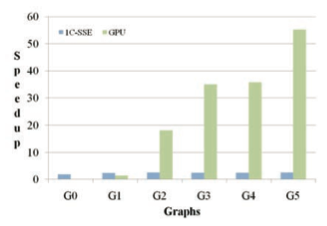
\includegraphics[width=\columnwidth]{images/speedups.png}
	\caption{Best results achieved (image from the original paper). The original caption states that these results reveal the speedup obtained with the CUDA implementation compared to the two sequential versions. Yet, the legend in the chart and the results text in the paper leads to the conclusion that these results are for the CUDA and SSE implementations against the C++ scalar O2 version.}
\end{figure}